\setlength\parindent{0pt}

\chapter{Background Theory}

\section{Battery Performace Testing}
There are a large number of factors that determine the battery usage of a device. Some of them are system level, including brightness, hardware power consumption and operating system battery consumption, which are beyond the control of application developers. However there exist a large number of factors such as CPU usage, network usage, wakelocks, etc which developers can look into, to optimize. \\

CPU usage results from performing computations. CPU usage is of two types, foreground usage, i.e when the app is running in the foreground, and background usage, for when app is running in the background (to perform tasks such as synchronisation, download, checking for mails, messages, etc). While foreground CPU usage forms a major part of battery consumption by cpu, if unchecked, a lot of unnecessary computation and processing maybe happening in the background, leading to battery drain (Unnecessary computation and processing may be taking place in the foreground as well) \\

Network usage, including mobile network and WiFi also form a major portion of battery usage. Like CPU usage, network usage is also of two types, background and foreground. Also like CPU usage, the app may be sending and receiving unnecessary packets in the foreground, background, or both. This is a potential candidate in making an app battery heavy.\\

Wakelock is a feature, which when requested by an app, lets the app to prevent the phone from going to sleep, i.e. the app will run continuously.\cite{wakelock} Wakelocks are handled differently in iOS and Android. While Android provides more control to the developer to invoke and use wakelocks through partial wakelocks, which lets apps run in the background, executing tasks, regardless of screen state or display timeouts, iOS permits partial wakelocks only for VOIP and location services.\cite{stackoverflow} It is pretty evident that an app requesting for unnecessary wakelocks will have a high energy consumption.\\

There may be external factors in an app’s battery consumption, such as bluetooth usage, camera usage or some other function whose power consumption is not directly controllable by the app. Such factors cannot be handled by the developers of the app, and hence such factors will not be taken into account. There may also arise unanticipated bugs in the app which lead to battery drain. 

\section{Automated UI Testing}
Test Automation has become one of the important aspects in the Software development world, especially in places where agile development strategies are followed. Mike Cohn has developed the Agile Test Automation Pyramid\cite{pyramid} as shown in figure 2.1:
\begin{figure}[!h]
 	\begin{center}
		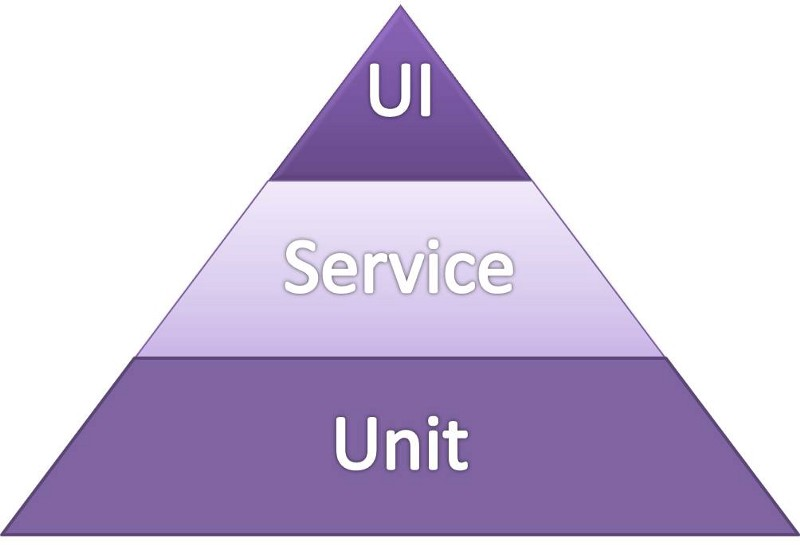
\includegraphics[scale=0.5]{pyramid}
		\caption{Agile Test Automation Pyramid}
	\end{center}
\end{figure}

Unit tests form the base of this pyramid. These are used to test the different components of the software and form the major part of automation testing. The Service level tests form the next layer. These deal with integrating all domain and functionality tools. The User Interface (UI) tests form the apex and are responsible for testing longer-running, core customer usage workflows

Below are a few cases in which UI test automation is valuable:
\begin{itemize}
	\item Regression Testing. Automation can free human testers of the boring and repeated process of regression testing.
	\item Testing applications which do not have unit tests developed. This helps to introduce automated testing in legacy applications.
	\item Cross-browser and Cross-platform testing. This is mostly executing the same tests on different versions. This is also the case for mobile applications for testing different OS versions and device models.
	\item Performance Testing as it requires a higher load than that manual testing cannot generate.

\end{itemize}
Following are some criteria for selecting test cases for automation:
\begin{itemize}
	\item Test cases which are frequently executed as part of smoke and regression
	\item Test cases which implement complex logic and calculations
	\item Test cases which need to be executed across multiple platforms
	\item Test cases where the manual execution can be difficult eg. Performance
\end{itemize}